\documentclass[12pt,a4paper]{article}
\usepackage[czech]{babel}
\usepackage[utf8]{inputenc} 
\usepackage{listings}
\lstset{language=C}
\usepackage{minted}
\usepackage[hidelinks]{hyperref}
\usepackage{graphicx}
\usepackage{caption}
\usepackage[all]{hypcap}
\usepackage{pdfpages}

\newcommand{\Csh}{C\#}

\renewcommand\listingscaption{Výpis}


\begin{document}
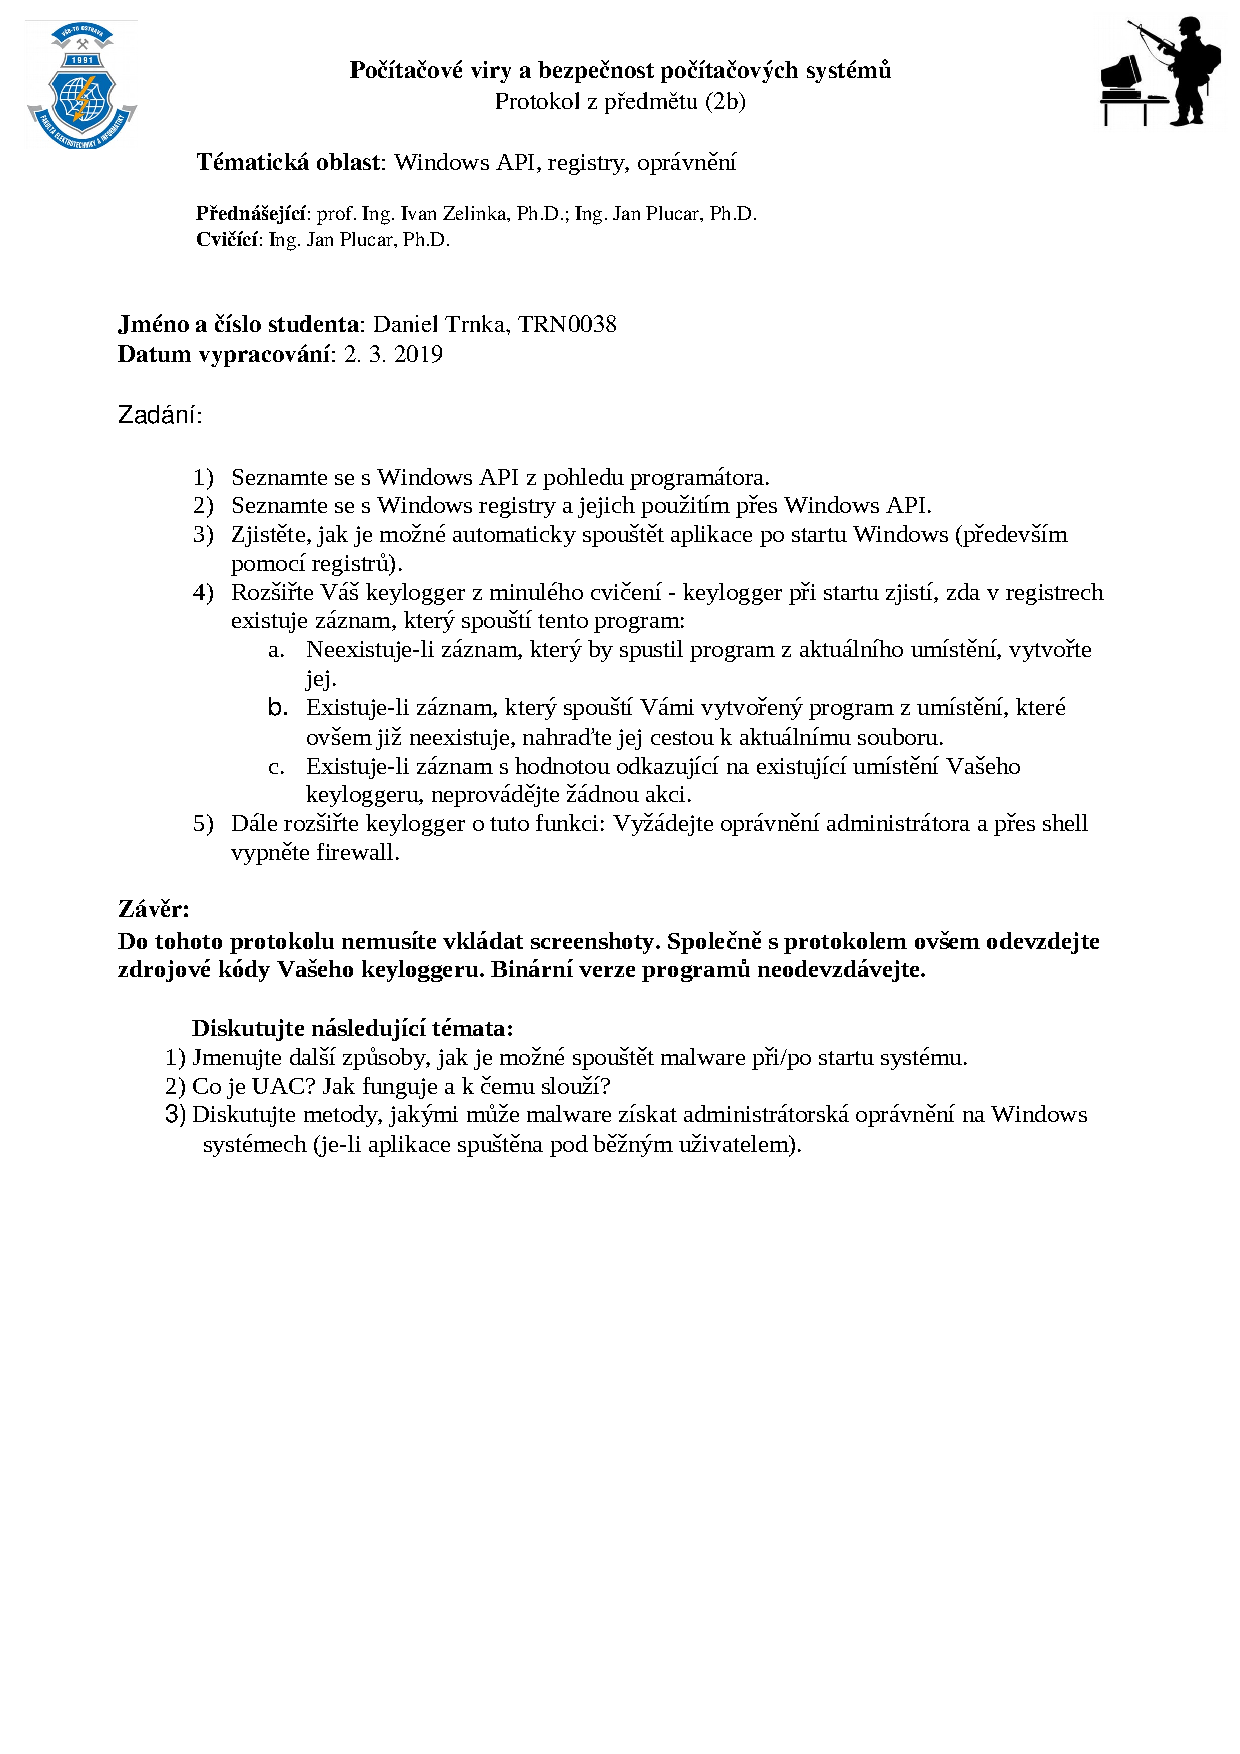
\includepdf[pages=1]{zadani.pdf}


Program z předchozího cvičení byl rozšířen o automatické spuštění po startu systému, resp. po přihlášení daného uživatele.
Existuje několik možností jak zajistit spouštění malware po startu systému.

První z možnosti, jak spustit program po přihlášení, je vytvořit v registrech nový klíč s prefixem \mint{html}|HKEY_CURRENT_USER\Software\Microsoft\Windows\CurrentVersion\Run| obsahující cestu k programu.
Stejná funkcionalita existuje i v \texttt{HKEY\_LOCAL\_MACHINE}, ale zápis vyžaduje administrátorské oprávnění, protože se aplikuje na všechny uživatele.

Další možnosti je zkopírovat soubor do startup adresáře, který je ve výchozím nastavení:
\mint{html}|%APPDATA%\Microsoft\Windows\Start Menu\Programs\Startup|

Využití služby není možné, protože lze nainstalovat hook pouze u procesů, které byly spuštěné ``interaktivním'' způsobem.

AppInit\_DLL umožňuje namapovat vlastní DLL knihovnu do všech interaktivních aplikací\footnote{https://docs.microsoft.com/en-us/windows/desktop/dlls/secure-boot-and-appinit-dlls}.
V adresáři \texttt{c} je zdrojový kód knihovny zachytávající klávesy, které jsou následně uloženy do souboru.
Procesy s \texttt{user32.dll} si danou knihovnu namapují a tím se zavolá funkce \texttt{DllMain}.
Funkce spustí nové vlákno a zaregistruje hook \texttt{WH\_KEYBOARD\_LL} ve kterém zachytnuté klávesy ukládá do souboru.

Aby se knihovna načítala v každém procesu tak je nutné v registrech upravit dva klíče s prefixem 
\mint{html}|HKEY_LOCAL_MACHINE\SOFTWARE\Microsoft\Windows NT \CurrentVersion\Windows|
Prvním klíčem je \texttt{AppInit\_DLLs}, který obsahuje cestu k DLL knihovně a druhý klič \texttt{LoadAppInit\_DLLs} musí být nastaven na hodnotu 1, aby byla tato funkcionalita povolena.
Změnu v registrech je nutné provést jako administrátor a systém musí nabootovat bez zapnutého SecureBoot.


Dalším úkolem bylo vypnout firewall.
V \Csh{} keyloggeru se spustí nový \texttt{powershell.exe} proces se skrytým oknem a v argumentech se předá skript z výpisu~\ref{lst:disable_fw}.
Skript prvně vyhledá zapnuté firewall profily.
Pokud nějaký zapnutý firewall existuje tak se spustí nový \texttt{powershell.exe} s administrátorským oprávněním a spustí se vypnutí firewallu.
Uživatel je tak pomocí UAC dotázán pouze v případě zapnutého firewallu.


\begin{listing}
	\begin{minted}{powershell}
$disabled = Get-NetFirewallProfile -All `
 | Where-Object -Property Enabled -EQ true `
 | measure;

if ($disabled.Count -gt 0) {
 echo "will disable firewall";
 Start-Process powershell `
  -WindowStyle Hidden `
  -Verb runAs `
  'Get-netFirewallProfile -All `
    | where Enabled -eq True `
    | foreach { Set-NetFirewallProfile -Profile $_.Name -Enabled false }';
}
	\end{minted}
	\caption{Powershell skript pro vypnutí firewallu dle potřeby}
	\label{lst:disable_fw}
\end{listing}


Aby se ztížila analýza programu, tak je daný powershell skript uložen v šifrované podobě, kde klíč se získá postupným zkoušením všech cest souborů na disku.
Ve zdrojových kódech se jedná o klíč \texttt{C:$\backslash$Windows$\backslash$explorer.exe}.
Touto metodou lze ale cílit na konkrétní skupinu počítačů na kterých se daný malware aktivuje a při běhu v sandboxu neposkytne žádná data.

Díky \textbf{User Account Control (UAC)} lze spouštět aplikace s nižším oprávněním a až dle potřeby se zobrazí potvrzovací dialogové okno pro udělení administrátorských práv.
Cílem je, aby aplikace neběžely s plnými právy a uživatel měl možnost případně odmítnout.
Ne vždy je ale dostatek informací k rozhodnutí zda povolit či ne - keylogger spouštěl nový proces \texttt{powershell.exe} s administrátorským oprávněním, ale v UAC dialogovém okně (obrázek~\ref{fig:uac}) bylo pouze zobrazena informace o powershell od Microsoft, což může působit důvěryhodně a navíc může jakákoliv legitimní aplikace pustit powershell.

\begin{figure}[ht]
	\centering
	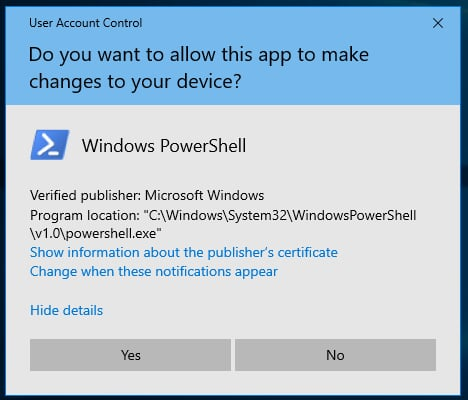
\includegraphics[width=9cm]{uac_powershell}
	\caption{UAC potvrzovací okno bez informacemi o předkovi, který daný proces vytvořil}
	\label{fig:uac}
\end{figure}

Aplikace běžící pod normálním uživatelem může naivně získat administrátorská oprávnění vytvořením nového procesu s \texttt{verb = runas}.
Ve výchozím nastavení však musí uživatel potvrdit UAC dialogové okno, neznalý uživatel však může automaticky vše potvrzovat.
V jazyce \Csh{} může spuštění procesu s administrátorským oprávněním vypadat následovně: 

\begin{minted}{csharp}
var proc = new ProcessStartInfo();
proc.FileName = "powershell.exe";
proc.Verb = "runas";
Process.Start(proc);
\end{minted}

Další možnosti by mohlo být využití programu \texttt{runas.exe}, ale vypadá to, že vyžaduje zadat heslo administrátora ručně.
Dále se může aplikace rovnou při spuštění zažádat o administrátorské oprávnění.
Lze to docílit přidáním manifestu z výpisu~\ref{lst:manifest}  do výsledného spustitelného souboru.

Dále lze například vyzkoušet zachytnutá hesla, zda nejsou použitá i pro administrátorský účet.
Využít špatně nakonfigurovaný systém - příliš volná přístupová práva do systémových adresářů.
Nebo využít nějakou chybu v systému.


\begin{listing}
\begin{minted}{xml}
<?xml version="1.0" encoding="UTF-8" standalone="yes"?>
<assembly xmlns="urn:schemas-microsoft-com:asm.v1" manifestVersion="1.0">
 <trustInfo xmlns="urn:schemas-microsoft-com:asm.v3">
  <security>
   <requestedPrivileges>
	<requestedExecutionLevel 
	  level="requireAdministrator"
	  uiAccess="false"/>
   </requestedPrivileges>
  </security>
 </trustInfo>
</assembly>
\end{minted}
\caption{Manifest pro zažádání administrátorského oprávnění hned při startu aplikace}
\label{lst:manifest}
\end{listing}

\end{document}